\documentclass[tikz, border=15pt]{standalone}
\usetikzlibrary{shapes, arrows.meta, positioning, backgrounds, fit}

\begin{document}
	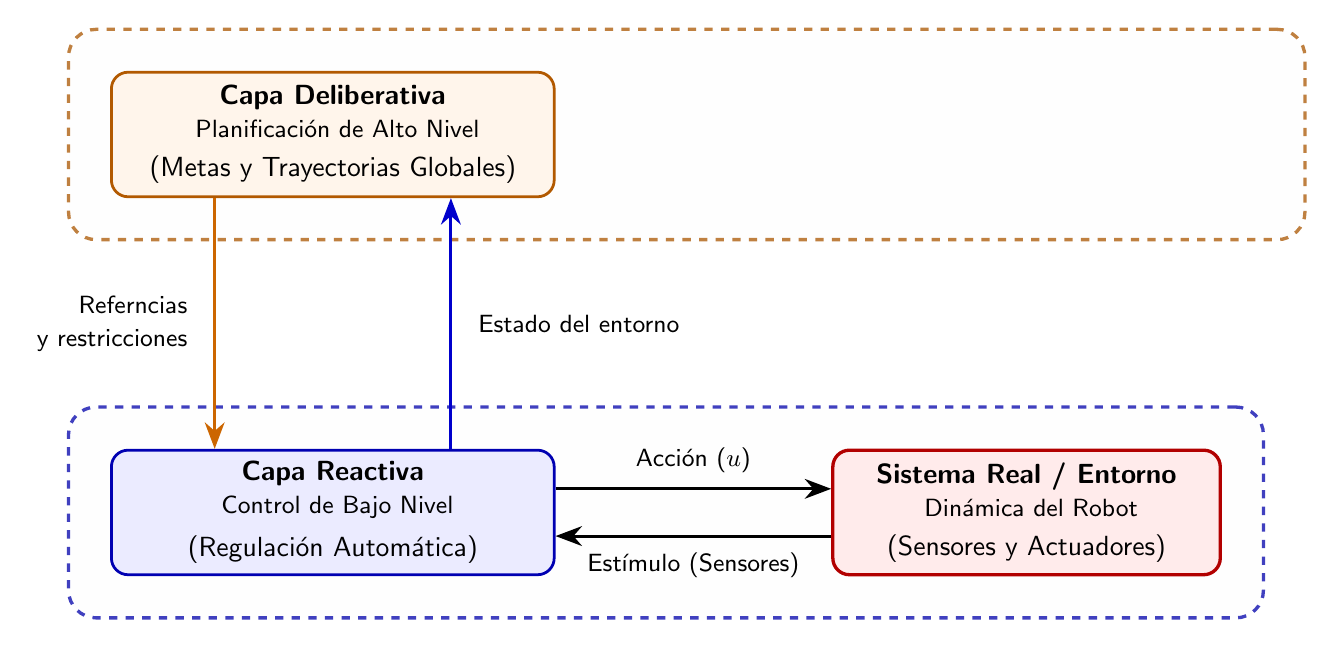
\begin{tikzpicture}[
		font=\sffamily,
		% --- ESTILOS DE LOS BLOQUES CRUCIALES ---
		block_delib/.style = {draw=orange!70!black, fill=orange!8!white, rectangle, minimum height=4.5em, minimum width=16em, align=center, rounded corners=6pt, line width=1pt},
		block_react/.style = {draw=blue!70!black, fill=blue!8!white, rectangle, minimum height=4.5em, minimum width=16em, align=center, rounded corners=6pt, line width=1pt},
		plant/.style = {draw=red!70!black, fill=red!8!white, rectangle, minimum height=4.5em, minimum width=14em, align=center, rounded corners=6pt, line width=1.2pt},
		% --- ESTILOS DE LOS CONTENEDORES DE FONDO ---
		layer_reactive/.style = {draw=blue!50!gray, fill=blue!5!gray!1, dashed, rounded corners=10pt, line width=1.2pt, inner sep=15pt},
		layer_deliberative/.style = {draw=orange!50!gray, fill=orange!5!gray!1, dashed, rounded corners=10pt, line width=1.2pt, inner sep=15pt},
		>={Stealth[scale=1.2]}
		]
		
		% =========================================================================
		% 1. POSICIONAMIENTO GEOMÉTRICO DE LOS BLOQUES
		% =========================================================================
		% Capa Superior
		\node [block_delib] (delib) at (0,0) {\textbf{Capa Deliberativa}\\ \vspace{0.2em} \small Planificación de Alto Nivel\\ (Metas y Trayectorias Globales)};
		
		% Capa Inferior (Separación vertical aumentada a 4.8cm para dar aire a los textos centrales)
		\node [block_react] (react) [below=4.8cm of delib.center, anchor=center] {\textbf{Capa Reactiva}\\ \vspace{0.2em} \small Control de Bajo Nivel\\ (Regulación Automática)};
		
		% Sistema Real / Entorno (Separación horizontal limpia a la derecha de la reactiva)
		\node [plant] (planta) [right=3.5cm of react] {\textbf{Sistema Real / Entorno}\\ \vspace{0.2em} \small Dinámica del Robot\\ (Sensores y Actuadores)};
		
		% =========================================================================
		% 2. FLUJOS DE INFORMACIÓN Y FLECHAS
		% =========================================================================
		% Canal de Bajada (Planes) - Desplazado a la izquierda
		\draw [->, line width=1.1pt, orange!80!black] ([xshift=-1.5cm]delib.south) -- 
		node[left, align=right, text=black, xshift=-6pt] {\small Referncias\\ \small y restricciones} 
		([xshift=-1.5cm]react.north);
		
		% Canal de Subida (Feedback síncrono) - Desplazado a la derecha
		\draw [->, line width=1.1pt, blue!80!black] ([xshift=1.5cm]react.north) -- 
		node[right, align=left, text=black, xshift=6pt] {\small Estado del entorno} 
		([xshift=1.5cm]delib.south);
		
		% Lazo Cerrado de Alta Velocidad (Horizontal entre Reactiva y Planta)
		\draw [->, line width=1.1pt] ([yshift=0.3cm]react.east) -- node[above, text=black, yshift=2pt] {\small Acción ($u$)} ([yshift=0.3cm]planta.west);
		\draw [->, line width=1.1pt] ([yshift=-0.3cm]planta.west) -- node[below, text=black, yshift=-2pt] {\small Estímulo (Sensores)} ([yshift=-0.3cm]react.east);
		
		% =========================================================================
		% 3. CAPAS DE FONDO Y TÍTULOS PROTEGIDOS
		% =========================================================================
		\begin{scope}[on background layer]
			% --- CAPA INFERIOR (REFLEJO MOTOR) ---
			% Forzamos un nodo auxiliar arriba a la derecha para que la caja envuelva de forma simétrica todo el espacio inferior
			\node[layer_reactive, fit=(react) (planta)] (reactive_bg) {};
			
			% Título Inferior colocado justo en la esquina superior interna
			\node[anchor=north west, font=\bfseries\sffamily\color{blue!80!black}, xshift=12pt, yshift=-8pt] 
			(title_react) at (reactive_bg.north west) {};
			
			% --- CAPA SUPERIOR (PROCESO CONSCIENTE) ---
			% Para que visualmente se extienda igual de ancho que la de abajo, usamos el alineamiento horizontal (-| planta.east)
			\coordinate (top_right) at ([xshift=15pt]delib.north -| planta.east);
			\node[layer_deliberative, fit=(delib) (top_right)] (deliberative_bg) {};
			
			% Título Superior colocado en su respectiva esquina
			\node[anchor=north west, font=\bfseries\sffamily\color{orange!80!black}, xshift=12pt, yshift=-8pt] 
			at (deliberative_bg.north west) {};
		\end{scope}
		
	\end{tikzpicture}
\end{document}